\documentclass[a4paper,11pt,twoside]{IT-CNEA}
\usepackage[utf8]{inputenc} % para cambiar el encoding
\usepackage{multicol}

%%%%%%%%%%%%%%%%%%%%%%%%%%%%%%%%%%%%%%%%%%%%%%%%%%%%%%%%%%%%%%%%%%%%%%%%%%%
%               Parametros principales del documento                      %
%%%%%%%%%%%%%%%%%%%%%%%%%%%%%%%%%%%%%%%%%%%%%%%%%%%%%%%%%%%%%%%%%%%%%%%%%%%

% Titulo
\titulo{Propagación de ruido en sistema LTI}
%
% Titulo alternativo para el encabezado
\alttitulo{Elementos de matemáticas aplicada para aplicaciones tecnlógicas}

% Autores
\autores{Augusto Conrado Sardá}{}

% Revisores
\revisores{Jose Relloso}{Agustín Casquero}{}

% Revision de calidad
\calidad{}

% Aprobacion
\aprobacion{}

%Objetivo
\objetivo{}
% Alcance
%\alcance{}

% Numero de informe tecnico
\numeroIT{TP Nº1}
% Metadatos para pdf
\hypersetup{
    pdfauthor={Augusto Conrado Sardá},
    pdftitle={AllanVariance},
    pdfkeywords={},
    pdfcreator={},
    pdfsubject={}    
    }
    
% Autores de revisiones
%\definechangesauthor[name={Johann Sebastian Mastropiero}, color=blue]{mas}
\usepackage{units}
\usepackage{fancyvrb}
\begin{document}
    % Creacion de la caratula
%    \portada    
    % Creacion del indice
    \tableofcontents       
    % Comienzo del desarrollo del documento
    \printnomenclature[2cm]

\clearpage  
\newpage
En las primeras simulaciones se pretende comprender la simulación del filtro de Kalman extendido multiplicativo (MEKF por sus siglas en inglés) brindada por la cátedra. 
\\ El modelo de giróscopo se simplifica, considerando sólo las componentes de angle random walk (ARW), rate random walk (RRW) y bias instability (BI). Para las primeras simulaciones se simplificó aún más haciendo $RRW=BI=0$, dejando sólo $ARW=0.015\,deg/\sqrt{h}$ (valor correspondiente a un giróscopo de tecnología ring laser gyro - RLG). También, se considera que posee un bias constante de $0.04\,deg/h\approx 0.19\,10^{-6}\,rad/s$. 
\begin{table}[h!]
\centering
\caption{Modelo del giróscopo para las simulaciones 1, 2 y 3}
\label{tabla:modeloGyroRLGSimulaciones123}
\begin{tabular}{|c|c|c|}
\hline
Parámetro & Unidad& Valor\\ \hline
ARW&$deg/\sqrt{h}$&$0.015$ \\ \hline
RRW&$deg/\left(h\sqrt{h}\right)$&$0$ \\ \hline
BI&$deg/h$&$0$ \\ \hline
Bias constante&$deg/h$&$0.04$ \\ \hline
%&&&&&& \\ \hline
\end{tabular}
\end{table}
\\ Respecto al modelo del star tracker (ST), se considera que posee una desviación estándar de $0.01\,deg$.
\\ En cuanto a la matriz $R$ involucrada en la actualización de la matriz $P$, se considera el mismo valor (en los tres ejes) del desvío estándar que en el modelo del ST. 
\\ Establecido este set (modelos del giróscopo y del ST, e inicialización de la matriz $R$) se realizaron tres simulaciones distintas variando el valor de la matriz $Q$, asociada a la propagación de la matriz $P$. 
\section{Simulación 1}
Para inicializar la matriz $Q$ se estableció $ARW=0.001\,deg/\sqrt{h}$ y $RRW=0.01\,deg/\left( h\sqrt{h}\right)$. El primero debería en teoría coincidir con el valor puesto para el modelo del giróscopo (tabla Nº\ref{tabla:modeloGyroRLGSimulaciones123}), pero se lo modificó bajo la consideración de que es difícil conocer cual es ARW que posee el sensor. Entonces, para inicializar la matriz $Q$ se utilizan valores que con algún criterio representen lo mejor posible al sensor (por lo general, este criterio se obtiene de la interpretación de la hoja de datos). Para el valor de RRW, el valor ingresado es bajo el criterio de que sea "suficientemente chico", puesto que no se puede inicializar $Q$ con RRW nulo. 
\par En las Figs. Nº\ref{fig:Simulacion1/KalmanQuaterion} y Nº\ref{fig:Simulacion1/KalmanBias} se observan la evolución de los valores de las ganancias Kalman asociadas a la estimación del cuaternión y del bias. El hecho de alcancen valores estacionarios es un comportamiento esperable del filtro de Kalman. De hecho, existen maneras de calcular estos valores estacionarios de las ganancias ignorando los transitorios. 
\\ En la Fig. Nº\ref{fig:Simulacion1/biasEstimado} se observa la evolución de la estimación del bias y como aproximadamente alrededor de $3000\,s$ converge al valor de bias constante establecido como parte del modelo del giróscopo. Esta convergencia no es estacionaria puesto que el esta sujeto a ruido (¡ruido que se pretende modelar con el modelo del giróscopo!). En la parte superior de la Fig. Nº\ref{fig:Simulacion1/biasEstimadoRMSErrores} se ha calculado el RMS del bias estimado a partir de $3000\,s$ y en la parte inferior el error de este respecto al valor de bias constante establecido. Una evaluación rápida de la Fig. Nº\ref{fig:Simulacion1/biasEstimadoRMSErrores} es que a partir de $3000\,s$, el RMS del bias estimado se encuentra alrededor del bias constante dentro del $9\%$ de error. 
\begin{figure}[h!]
\centering
\includegraphics[width=18cm]{/home/pelotari/Documents/MaestriaIB/Materias/ElementosMatematicaGit/TP2Kalman/SimulacionesV2/Simulacion1/KalmanQuaterion.png}
\caption{Simulación 1: Ganancias de Kalman asociadas al cuaternión estimado}
\label{fig:Simulacion1/KalmanQuaterion}
\end{figure}
\begin{figure}[h!]
\centering
\includegraphics[width=18cm]{/home/pelotari/Documents/MaestriaIB/Materias/ElementosMatematicaGit/TP2Kalman/SimulacionesV2/Simulacion1/KalmanBias.png}
\caption{Simulación 1: Ganancias de Kalman asociadas al bias estimado}
\label{fig:Simulacion1/KalmanBias}
\end{figure}
\begin{figure}[h!]
\centering
\includegraphics[width=18cm]{/home/pelotari/Documents/MaestriaIB/Materias/ElementosMatematicaGit/TP2Kalman/SimulacionesV2/Simulacion1/biasEstimado.png}
\caption{Simulación 1: Bias estimado}
\label{fig:Simulacion1/biasEstimado}
\end{figure}
\begin{figure}[h!]
\centering
\includegraphics[width=18cm]{/home/pelotari/Documents/MaestriaIB/Materias/ElementosMatematicaGit/TP2Kalman/SimulacionesV2/Simulacion1/biasEstimadoRMSErrores.png}
\caption{Simulación 1: RMS del bias estimado y error respecto del bias constante}
\label{fig:Simulacion1/biasEstimadoRMSErrores}
\end{figure}
\begin{figure}[h!]
\centering
\includegraphics[width=18cm]{/home/pelotari/Documents/MaestriaIB/Materias/ElementosMatematicaGit/TP2Kalman/SimulacionesV2/Simulacion1/erroresQuaterniones.png}
\caption{Simulación 1: Errores de los cuaterniones medido y estimado respecto al \textit{real}.}
\label{fig:Simulacion1/erroresQuaterniones}
\end{figure}
\section{Simulación 2}
En esta simulación se inicializa la matriz $Q$ con $ARW=0.001*9\,deg/\sqrt{h}$ y RRW no se modifica. 
\par Las Figs. Nº\ref{fig:Simulacion2/KalmanQuaterion} y Nº\ref{fig:Simulacion2/KalmanBias} se muestran las evoluciones de las ganancias de Kalman. En comparación con las Figs. Nº\ref{fig:Simulacion1/KalmanQuaterion} y Nº\ref{fig:Simulacion1/KalmanBias}, los valores estacionarios de esta segunda simulación resultan mayores a los primeros. Puesto que el filtro propaga valiéndose de la medición del giróscopo, al incrementar ARW en la matriz $Q$ se le está ``indicando'' al filtro que se tiene mayor incertidumbre en la medición de este. Por lo tanto el filtro le dará mayor importancia a la actualización que a la propagación y por lo tanto los valores de las ganancias de Kalman aumentarán. 
\\ En cuánto a la estimación del bias del giróscopo, aproximadamente alrededor de $400\,s$ se observa que converge al valor de bias constante. Por lo tanto, el cálculo del RMS del bias estimado se realizó a partir de este tiempo. En comparación con la simulación anterior es claro como aumentó el porcentaje de error en consecuencia de indicarle al filtro que la incerteza en la medición del giróscopo es mayor. 
% Q 
% q
\begin{figure}[h!]
\centering
\includegraphics[width=18cm]{/home/pelotari/Documents/MaestriaIB/Materias/ElementosMatematicaGit/TP2Kalman/SimulacionesV2/Simulacion2/KalmanQuaterion.png}
\caption{Simulación 2:  Ganancias de Kalman asociadas al cuaternión estimado}
\label{fig:Simulacion2/KalmanQuaterion}
\end{figure}
\begin{figure}[h!]
\centering
\includegraphics[width=18cm]{/home/pelotari/Documents/MaestriaIB/Materias/ElementosMatematicaGit/TP2Kalman/SimulacionesV2/Simulacion2/KalmanBias.png}
\caption{Simulación 2:  Ganancias de Kalman asociadas al bias estimado}
\label{fig:Simulacion2/KalmanBias}
\end{figure}
\begin{figure}[h!]
\centering
\includegraphics[width=18cm]{/home/pelotari/Documents/MaestriaIB/Materias/ElementosMatematicaGit/TP2Kalman/SimulacionesV2/Simulacion2/biasEstimado.png}
\caption{Simulación 2:  Bias estimado}
\label{fig:Simulacion2/biasEstimado}
\end{figure}
\begin{figure}[h!]
\centering
\includegraphics[width=18cm]{/home/pelotari/Documents/MaestriaIB/Materias/ElementosMatematicaGit/TP2Kalman/SimulacionesV2/Simulacion2/biasEstimadoRMSErrores.png}
\caption{Simulación 2:  RMS del bias estimado y error respecto del bias constante}
\label{fig:Simulacion2/biasEstimadoRMSErrores}
\end{figure}
\begin{figure}[h!]
\centering
\includegraphics[width=18cm]{/home/pelotari/Documents/MaestriaIB/Materias/ElementosMatematicaGit/TP2Kalman/SimulacionesV2/Simulacion2/erroresQuaterniones.png}
\caption{Simulación 2:  Errores de los cuaterniones medido y estimado respecto al \textit{real}.}
\label{fig:Simulacion2/erroresQuaterniones}
\end{figure}
\section{Simulación 3}
Para finalizar con este primero juego de simulaciones, ahora se disminuyo ARW en la matriz $Q$ a $ARW=0.001/9\,deg/\sqrt{h}$.
\\ En este caso las ganancias de Kalman alcanzan valores inferiores respecto a las Figs. Nº\ref{fig:Simulacion1/KalmanQuaterion} y Nº\ref{fig:Simulacion1/KalmanBias}. La explicación es la opuesta que en la simulación 2. Ahora, al comunicarle al filtro que se tiene menor incerteza en la medición del giróscopo, la propagación es más significativa y por lo tanto las ganancias de Kalman disminuyen. 
\\ Repecto a la estimación del bias, se tiene un tiempo de convergencia considerablemente mayor. Para calcular el RMS de la Fig. Nº\ref{fig:Simulacion3/biasEstimadoRMSErrores} se tomó a partir de $24000\,s$. Sin embargo, aunque el tiempo de convergencia es mayor, el error disminuye significativamente. 
%Q
%q
\begin{figure}[h!]
\centering
\includegraphics[width=18cm]{/home/pelotari/Documents/MaestriaIB/Materias/ElementosMatematicaGit/TP2Kalman/SimulacionesV2/Simulacion3/KalmanQuaterion.png}
\caption{Simulación 3:  Ganancias de Kalman asociadas al cuaternión estimado}
\label{fig:Simulacion3/KalmanQuaterion}
\end{figure}
\begin{figure}[h!]
\centering
\includegraphics[width=18cm]{/home/pelotari/Documents/MaestriaIB/Materias/ElementosMatematicaGit/TP2Kalman/SimulacionesV2/Simulacion3/KalmanBias.png}
\caption{Simulación 3:  Ganancias de Kalman asociadas al bias estimado}
\label{fig:Simulacion3/KalmanBias}
\end{figure}
\begin{figure}[h!]
\centering
\includegraphics[width=18cm]{/home/pelotari/Documents/MaestriaIB/Materias/ElementosMatematicaGit/TP2Kalman/SimulacionesV2/Simulacion3/biasEstimado.png}
\caption{Simulación 3:  Bias estimado}
\label{fig:Simulacion3/biasEstimado}
\end{figure}
\begin{figure}[h!]
\centering
\includegraphics[width=18cm]{/home/pelotari/Documents/MaestriaIB/Materias/ElementosMatematicaGit/TP2Kalman/SimulacionesV2/Simulacion3/biasEstimadoRMSErrores.png}
\caption{Simulación 3:  RMS del bias estimado y error respecto del bias constante}
\label{fig:Simulacion3/biasEstimadoRMSErrores}
\end{figure}
\begin{figure}[h!]
\centering
\includegraphics[width=18cm]{/home/pelotari/Documents/MaestriaIB/Materias/ElementosMatematicaGit/TP2Kalman/SimulacionesV2/Simulacion3/erroresQuaterniones.png}
\caption{Simulación 3:  Errores de los cuaterniones medido y estimado respecto al \textit{real}.}
\label{fig:Simulacion3/erroresQuaterniones}
\end{figure}
\section{Simulación 4}
En esta simulación se cambia el modelo del giróscopo por uno de tecnología MEMS, aunque se continúa con la simplificación que RRW y BI son nulos. En la tabla Nº\ref{tabla:modeloGyroRLGSimulacion4} se muestran los valores de los parámetros. Y respecto al modelo del ST, este no sufre modificaciones. 
\\ En cuanto a las matrices  $R$ y $Q$, la primera tampoco cambia mientras que la segunda si. Se estable $ARW=3\,deg/\sqrt{h}$ y $RRW=10\,deg/\left( h\sqrt{h}\right)$. En primera instancia se había optado por valores de RRW menores, pero se incurría en tiempos de simulación excesivamente largos.
\begin{table}[h!]
\centering
\caption{Modelo del giróscopo para la simulación 4}
\label{tabla:modeloGyroRLGSimulacion4}
\begin{tabular}{|c|c|c|}
\hline
Parámetro & Unidad& Valor\\ \hline
ARW&$deg/\sqrt{h}$&$1.8$ \\ \hline
RRW&$deg/\left(h\sqrt{h}\right)$&$0$ \\ \hline
BI&$deg/h$&$0$ \\ \hline
Bias constante&$deg/h$&$0.25$ \\ \hline
%&&&&&& \\ \hline
\end{tabular}
\end{table}
\par Como indican los parámetros de la tabla Nº\ref{tabla:modeloGyroRLGSimulacion4}, este tipo de giróscopo es de menor calidad que el RLG. A su vez, con la inicialización dada para la matriz $Q$, las ganancias de Kalman para el cuaternión (Fig. Nº\ref{fig:Simulacion4/KalmanQuaterion}) convergen al cabo de un periodo de muestreo del ST. También, los valores estacionarios de las ganancias de Kalman (Figs. Nº\ref{fig:Simulacion4/KalmanQuaterion} y Nº\ref{fig:Simulacion4/KalmanBias}) son del orden de 1000 veces mayor que en el caso de la simulación. Esto concuerda con el comportamiento que al ser un peor giróscopo, la actualización de la medición del ST del filtro cobra mayor importancia que la propagación mediante el modelo. 
\\ La Fig. Nº\ref{fig:Simulacion4/biasEstimadoRMSErrores} muestra claramente como la peor calidad del giróscopo ha degradado la estimación del bias. De los valores establecidos en la matriz $Q$, puede considerarse que ARW esté sobredimensionado, pero también al poner un alto valor de RRW para ``acelerar'' la convergencia se aumenta el error. Como puede observarse, el valor RMS fluctúa dentro del $80\%$ de error, lo que resulta inadmisible. Finalmente, la Fig. Nº\ref{fig:Simulacion4/erroresQuaterniones} se ratifica el mal desempeño ya que practicamente no hay diferencia entre el error del cuaternión estimado y el medido respecto del real. 
\section{Simulación 5}
%Q
%q
\begin{figure}[h!]
\centering
\includegraphics[width=18cm]{/home/pelotari/Documents/MaestriaIB/Materias/ElementosMatematicaGit/TP2Kalman/SimulacionesV2/Simulacion4/KalmanQuaterion.png}
\caption{Simulación 4:  Ganancias de Kalman asociadas al cuaternión estimado}
\label{fig:Simulacion4/KalmanQuaterion}
\end{figure}
\begin{figure}[h!]
\centering
\includegraphics[width=18cm]{/home/pelotari/Documents/MaestriaIB/Materias/ElementosMatematicaGit/TP2Kalman/SimulacionesV2/Simulacion4/KalmanBias.png}
\caption{Simulación 4:  Ganancias de Kalman asociadas al bias estimado}
\label{fig:Simulacion4/KalmanBias}
\end{figure}
\begin{figure}[h!]
\centering
\includegraphics[width=18cm]{/home/pelotari/Documents/MaestriaIB/Materias/ElementosMatematicaGit/TP2Kalman/SimulacionesV2/Simulacion4/biasEstimado.png}
\caption{Simulación 4:  Bias estimado}
\label{fig:Simulacion4/biasEstimado}
\end{figure}
\begin{figure}[h!]
\centering
\includegraphics[width=18cm]{/home/pelotari/Documents/MaestriaIB/Materias/ElementosMatematicaGit/TP2Kalman/SimulacionesV2/Simulacion4/biasEstimadoRMSErrores.png}
\caption{Simulación 4:  RMS del bias estimado y error respecto del bias constante}
\label{fig:Simulacion4/biasEstimadoRMSErrores}
\end{figure}
\begin{figure}[h!]
\centering
\includegraphics[width=18cm]{/home/pelotari/Documents/MaestriaIB/Materias/ElementosMatematicaGit/TP2Kalman/SimulacionesV2/Simulacion4/erroresQuaterniones.png}
\caption{Simulación 4:  Errores de los cuaterniones medido y estimado respecto al \textit{real}.}
\label{fig:Simulacion4/erroresQuaterniones}
\end{figure}
%Q
%q
\clearpage
\newpage
\bibliographystyle{asmems4}
\bibliography{biblio}
\end{document}
%\begin{figure}[h!]
%\centering
%\includegraphics[width=8cm]{Figuras/.png}
%\caption{}
%\label{fig:}
%\end{figure}
%\begin{figure*}[t!]
%    \centering
%    \begin{subfigure}[t]{0.5\textwidth}
%        \centering
%        \includegraphics[width=8cm]{Figuras/.png}
%        \caption{}
%        \label{fig:}
%    \end{subfigure}%
%    \begin{subfigure}[t]{0.5\textwidth}
%        \centering
%        \includegraphics[width=8cm]{Figuras/.png}
%        \caption{}
%        \label{fig:}
%    \end{subfigure}%
%    ~ 
%    \caption{}
%    \label{}
%\end{figure*}
%\begin{table}[h!]
%\centering
%\caption{}
%\label{tabla:}
%\begin{tabular}{|c|c|c|}
%\hline
%
%%&&&&&& \\ \hline
%\end{tabular}
%\end{table}


%que